% Beginning code for all standard physics latex documents

%Created on: May 8, 2014    Edited by: Wesley Kyle
%Edited on:	May 12, 2016	Edited by: P. Gimby - cleaned up the code to remove unneeded packages
%Edited on:	May 13, 2016	Edited by: P. Gimby - collected a few more packages used in 325.
%Edited on:	May 16, 2016	Edited by: P. Gimby - fixed page numbering error.
%Edited on: May 20, 2016	Edited by: Alex Shook - Added packages for 497

\documentclass[justified]{tufte-book}
\usepackage{graphicx} % allow embedded images
\setkeys{Gin}{width=\linewidth,totalheight=\textheight,keepaspectratio}
\usepackage{amsmath}  % extended mathematics
\usepackage{bm}  % bold font in math mode
\usepackage{longtable} %lets long tables flow into multiple pages instead of running off the page or having to break tables up manually
\usepackage{booktabs} % book-quality tables
\usepackage{units}    % non-stacked fractions and better unit spacing
\usepackage{multicol} % multiple column layout facilities
\usepackage{tikz} %for drawing nice pictures
\usepackage{indentfirst} % makes first line of each new section be indented
\usepackage{enumitem} % extended options for the enumerate environment
\usepackage{soul} % gives more typestting options like spacing, underline, and strike-through
\usepackage{marvosym} %extra symbols package
\usepackage{multirow} % for special table controls
\usepackage[singlelinecheck=false]{caption} % allow captions w/o figure number
\captionsetup{compatibility=false} % corrects in issue with the caption package
\usepackage{float} % allows for contorl over position of figures and tables
\allowdisplaybreaks % allows equations to span two pages if needed
\usepackage{mathrsfs} % fancy math symbols
\usepackage{multirow} % for special table controls
\usetikzlibrary{arrows,shapes,snakes,calc,patterns,3d} % addon to tikz
\usetikzlibrary{circuits.ee.IEC} % addon to tikz
\usepackage{pgfplots} % package for making plots of functions
\usepackage{gensymb} % symbols i,e. degrees
\usetikzlibrary{decorations.pathmorphing} % to draw the springs
\tikzset{circuit declare symbol = ac source}
\tikzset{set ac source graphic = ac source IEC graphic}
\usepackage{changepage} % allows for full page environment
\usepackage{comment} % allows comment tags for large sections

% define new page style that puts page numbers in the middle
%\begin{comment}
\fancypagestyle{custom}{
\fancyhf{} % clear all header and footer fields
\fancyheadoffset{0pt}
\fancyfootoffset{0pt}
\fancyfoot[C]{\thepage}
\renewcommand{\headrulewidth}{0pt}
\renewcommand{\footrulewidth}{0pt}}
\pagestyle{custom}
%\end{comment}

%below creates a new circuit symbol for AC sources
\tikzset{
         ac source IEC graphic/.style=
          {
           transform shape,
           circuit symbol lines,
           circuit symbol size = width 3 height 3,
           shape=generic circle IEC,
           /pgf/generic circle IEC/before background=
            {
             \pgftransformresetnontranslations
             \pgfpathmoveto{\pgfpoint{-0.8\tikzcircuitssizeunit}{0\tikzcircuitssizeunit}}
             \pgfpathsine{\pgfpoint{0.4\tikzcircuitssizeunit}{0.4\tikzcircuitssizeunit}}
             \pgfpathcosine{\pgfpoint{0.4\tikzcircuitssizeunit}{-0.4\tikzcircuitssizeunit}}
             \pgfpathsine{\pgfpoint{0.4\tikzcircuitssizeunit}{-0.4\tikzcircuitssizeunit}}
             \pgfpathcosine{\pgfpoint{0.4\tikzcircuitssizeunit}{0.4\tikzcircuitssizeunit}}
             \pgfusepathqstroke
            }
          }
        }
% end of circuit symbol
%\begin{document}
%%%end individual beginning code/,$d


%  \begin{titlepage}
%    \vspace*{\fill}
%    \begin{center}
%      \huge{{\bf TITLE1}}\\[0.4cm]
%      \huge{TITLE2}\\[0.4cm]
%      \LARGE{Laboratory Manual}\\[0.4cm]
%      \large{SEASON YEAR}
%    \end{center}
%    \vspace*{\fill}
%  \end{titlepage}
%\maketitle

%\begin{spacing}{0.5}
%\tableofcontents
%\end{spacing}

%NEW PHYS 497 PACKAGES AND COMMANDS

%Subcaption package: Allows subfigures to be placed side by side, and labeled with individual captions (Added June 1, 2016)
\usepackage{subcaption}

%Array package: Allows for addiation specifications in arrays (Added May 6, 2016)
\usepackage{array}

%newcolumntype: Allows one to specify a fixed column width (Added May 6, 2016)
\newcolumntype{L}[1]{>{\raggedright\let\newline\\\arraybackslash\hspace{0pt}}m{#1}}
\newcolumntype{C}[1]{>{\centering\let\newline\\\arraybackslash\hspace{0pt}}m{#1}}
\newcolumntype{R}[1]{>{\raggedleft\let\newline\\\arraybackslash\hspace{0pt}}m{#1}}

%circuits.logic.US, circuits.logic.IEC: For drawing logic gates in Tikz (Added May 6, 2016) 
\usetikzlibrary{circuits.logic.US,circuits.logic.IEC}

\newcommand{\PGT}{ %PGT: positive going transition
\begin{tikzpicture}
\draw[-angle 60] (0,0) -- (0,5pt);
\draw (0,5pt) -- (0,6pt) -- (5pt,6pt);
\draw (-5pt,0) -- (0,0);
\end{tikzpicture}
}





%TEST
\usepackage{geometry}
\pagestyle{fancy}

%\usepackage[caption=false]{subfig}

%\makeatletter
%\renewenvironment{figure}[1][htbp]{%
%  \@tufte@orig@float{figure}[#1]%
%}{%
%  \@tufte@orig@endfloat
%}

%\renewenvironment{table}[1][htbp]{%
%  \@tufte@orig@float{table}[#1]%
%}{%
%  \@tufte@orig@endfloat
%}
%\makeatother

% use instead of subfigure
\makeatletter
\newenvironment{multifigure}[1][htbp]{%
  \@tufte@orig@float{figure}[#1]%
}{%
  \@tufte@orig@endfloat
}
\makeatother

\makeatletter
\newenvironment{mainfigure}[1][htbp]{%
\@tufte@orig@float{figure}[#1]
\begin{adjustwidth}{}{-153pt}}
{\end{adjustwidth}\@tufte@orig@endfloat}%
\makeatother

\makeatletter
\newenvironment{maintable}[1][htbp]{%
\@tufte@orig@float{table}[#1]
\begin{adjustwidth}{}{-153pt}}
{\end{adjustwidth}\@tufte@orig@endfloat}%
\makeatother

%%%% Labatorial Cross-over labs need this code. This should be temporary PG Dec 7, 2016

\newcounter{questioncounter}
\setcounter{questioncounter}{0}
\newcounter{checkpointcounter}
\setcounter{checkpointcounter}{0}
\newcounter{figurecounter}
\setcounter{figurecounter}{0}
%%%%%%%%%%%%%%%%%%%%%%%%%%%%%%%%%%%%%%%%%%%%%%%%%%%%%%%

\newcommand{\checkpoint}{
 \fbox{\begin{minipage}{0.2\textwidth}
 %\includegraphics[width=0.5\textwidth]{stop}
 \end{minipage}
 \begin{minipage}{1.0\textwidth}
 {\bf CHECKPOINT \addtocounter{checkpointcounter}{1} \arabic{checkpointcounter}: Before moving on to the next part, have your TA check the results you obtained so far.}
 \end{minipage}}}

%%% end labatorial cross-over code.

% New environment for placing figure captions under the figure
%\makeatletter
%\newenvironment{mainfigure}{\textwidth}[1][htbp]{%
%\@tufte@orig@float{figure}[#1]%
%}{%
%\@tufte@orig@endfloat
%}
%\makeatother

\begin{document}
%%%%%%%%%%%%%%%%%%%%%%%%%%%%%%%%%%%%%%%%%%%%%
%
% 0062 PHYS397FA2017
%
%%%%%%%%%%%%%%%%%%%%%%%%%%%%%%%%%%%%%%%%%%%%%


\setcounter{chapter}{4}
\setcounter{equation}{0}
\setcounter{table}{0}
\setcounter{figure}{0}
\chapter{Traveling Waves}

\section{Equipment}

% first column
\begin{minipage}[t]{0.5\textwidth}
\begin{itemize}[noitemsep]
\item Tek 2225 oscilloscope with BNC feedthrough termination
\item HP 8011A pulse generator
\item Fluke multimeter
\item 10 meter RG58 coaxial cable
\item 7 meter RG59 coaxial cable
\item 7 meter twinaxial cable
\item reflectionless signal splitter
\end{itemize}
\end{minipage}
%second column
\begin{minipage}[t]{0.5\textwidth}
\begin{itemize}[noitemsep]
\item 0.5 meter RG58 coaxial cable
\item BNC male-male adapter (2)
\item BNC female-female adapter
\item male BNC to female banana adapter
\item banana connecting cables (2)
\item variable resistive termination
\item short circuit termination
\end{itemize}
\end{minipage}

\begin{marginfigure}[+2in]
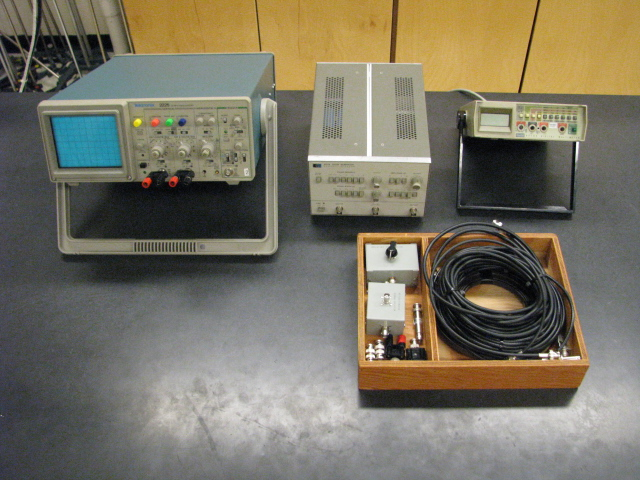
\includegraphics{/usr/local/master/labs/physics397-FA2017/0062-PHYS397FA2017/Travelling-Waves-Setup.jpg}
\caption{A photograph of the experimental setup.}
\label{fig:TWsetup}
\end{marginfigure}

\section{Preparation}
Review reflections of waves in ropes and study basic properties of the wave equation.

\section{Goals of the Experiment}
\begin{itemize}
    \item To understand the properties of traveling waves.
    \item To gain experience with pulse and timing measurements using an oscilloscope.
    \item To investigate physical situations where properties of traveling waves are applied.
\end{itemize}
%To understand some ideas and properties of traveling waves and gain experience with pulse and timing measurements using an oscilloscope. Also, to appreciate the wide range of physical situations where traveling wave ideas apply. 

\section{Theory}
Imagine a rope fixed to a wall and under tension at the free end. When this free end is flipped upwards once a wave travels down the rope until it reaches the wall. Here, the wave exerts a force on the wall and the wall exerts an equal and opposite force on the rope. The result is a wave opposite to the original wave traveling back on the rope in the reverse direction. The incident wave has been {\bf reflected} by the wall. As a second example, suppose now that one end of the rope is free to move up and down because it has been connected to a ring that is free to slide on a frictionless rod perpendicular to the rope. Now, when the free end is flipped up once, a wave travels down the rope as before. When this wave reaches the ring the force of the wave raises the ring which then falls back down to generate a wave travelling back down the rope. Unlike the solid wall, this wave is identical to the original wave, instead of opposite.

These two examples demonstrate that a wave on a rope is reflected by both a {\bf fixed rope termination} as well as a {\bf free rope termination}. The fixed and free rope ends are the extreme cases. In an intermediate case, where the rope termination is partly free (or partly fixed), the incident wave will be reflected back with varying intensities and can be opposite or identical, depending on whether the termination is closer to a free end or a fixed end. This logically implies there must be one termination exactly in between which produces no reflection. This {\bf proper termination} occurs when the rope end has a resistance to the wave that is exactly the same as the resistance of the rope itself. From the point of view of the rope, the wave continues onward without interruption because the wave only sees more identical rope ahead. From the point of view of an external observer, the proper termination has absorbed the wave and produced no reflection. This single value of resistance that absorbs waves instead of reflecting them is called the {\bf characteristic impedance}, $Z_0$. If the rope were thinner or more compliant the characteristic impedance would change. 

A second wave property of the rope is the velocity at which the wave propagates along the rope. Giving a harder flip will increase the height of the wave but it will not travel down the rope any faster. This {\bf velocity of propagation}, $V_p$, is dependent on the thickness and compliance of the rope. One can image reversing the rope so the formerly terminated end is now the end to be flipped. The waves will propagate and reflect on the rope the same as before. For the rope then, the characteristic impedance and velocity of propagation are identical for the the forward traveling waves and the reverse traveling reflected waves.

What happens if the rope is flipped twice so that the reflected wave from the first flip must cross the incoming wave of the second flip? The result is determined by a third property of the rope called the {\bf principle of superposition}. This principle states that when two waves overlap, the resulting vertical displacement of the rope (the height or {\bf amplitude}), is the sum of the individual displacements of each wave. The waves themselves do not interfere with each other. After the waves have crossed, each carries on as before without any change in speed or amplitude.

If the rope were ideal, or {\bf lossless}, then the traveling waves would never lose any energy. In practice, a wave traveling on a rope loses a constant fraction of its amplitude per meter of travel along the rope. This {\bf attenuation}, or {\bf loss factor}, of the rope is a fourth characteristic  property of the rope. Due to attenuation, a wave traveling on a very long rope will slowly decay away. In this experiment you will be observing and verifying each of these four properties.

The waves on a rope are an example of a mechanical traveling wave. Traveling wave phenomena occur in any situation where the travel time of a wave along the medium is significantly larger than the size of the wave. Examples of this are everywhere. Bats use acoustic traveling waves in air to locate their prey and avoid obstacles. Dolphins and submarines do the same with acoustic waves in water. The wake from a boat generates surface traveling waves on top of the water that take some time to reach the shore. Striking a hammer on a steel beam generates traveling waves in a solid medium. A sudden application and removal of heat generates a heat wave that travels by conduction. The sudden diffusion that occurs when one material is added to another is also a traveling wave. Lastly, electrical signals in wires and electromagnetic waves in space furnish many examples of traveling waves.

The size and speed of a traveling wave system can vary greatly. The yearly thermal cycle on a concrete dam generates waves with widths in the tens of meters. On the other hand, in a high frequency radar set the waves travel millimeters in a few nanoseconds. This experiment will examine electrical pulses in cables several meters long. The waves will travel the length of the cable in several tens of nanoseconds. This system is used for traveling wave experiments because it closely approximates an ideal traveling wave system. Furthermore, it is easy and fast to make direct measurements on the traveling waves and the cables are small and easily handled. This experiment would not be so easy to perform with yearly thermal waves in a concrete dam.

Let x be the position of the wave and t the time. Then all lossless linear traveling wave systems obey the {\bf telegrapher's equations}

\begin{equation}
\dfrac{\partial v}{\partial x}=-\dfrac{Z_0}{V_p}\cdot\dfrac{\partial i}{\partial t}
\label{equ:tw1}
\end{equation}

\noindent and

\begin{equation}
\dfrac{\partial i}{\partial x}=-\dfrac{1}{V_pZ_0}\cdot\dfrac{\partial v}{\partial t}
\label{equ:tw2}
\end{equation}

Since this experiment deals with electrical pulses on a cable, the variable $v$ represents the voltage and the variable $i$ represents the current. For any other traveling wave system they would represent some other relevant physical quantities. The partial derivatives are required because the wave depends on both the position and the time. Hence the voltage, $v$, is really a function $v(x,t)$, and the current, $i$, is really a function $i(x,t)$. The solutions to the telegraphers equations are

\begin{equation}
v(x,t)=f(x-V_pt)+g(x+V_pt)
\label{equ:tw3}
\end{equation}

\noindent and

\begin{equation}
i(x,t)=\dfrac{1}{Z_0}\left[f(x-V_pt)-g(x+V_pt)\right]
\label{equ:tw4}
\end{equation}

The solution functions $f$ and $g$ are {\bf arbitrary}. This means it does not matter what shape the traveling wave may have, the general behaviour remains unchanged.  Both the $f$ and $g$ functions each satisfy the telegrapher's equations alone. The reason for this is that $f$ and $g$ are arbitrary, so either $f$ or $g$ could be identically zero. This allows us to examine $f$ and $g$ independently. For $f$, as long as $x$ is increased with velocity, $V_p$ , the value of $f(x,t)$ remains unchanged. So $f$ is a wave traveling in the positive $x$ direction. Similarly, $g$ is a wave traveling in the negative $x$ direction. Set $g $to zero so the forward wave can be examined. Dividing Equation \ref{equ:tw3} by Equation \ref{equ:tw4} gives

\begin{equation}
\dfrac{v(x,t)}{i(x,t)}=Z_0
\label{equ:tw5}
\end{equation}

\noindent which is a travelling wave version of Ohm's law. For the reverse wave g, the result is

\begin{equation}
\dfrac{v(x,t)}{i(x,t)}=-Z_0
\label{equ:tw6}
\end{equation}

It is now possible to describe reflections quantitatively. Imagine a wave traveling on a cable that is terminated in a load $Z_T$ and has a characteristic impedance $Z_0$. Let $v^+$ be the voltage traveling toward the load and $v^-$ be the voltage reflected from the load. The voltage at the load (terminated end) must be

\begin{equation}
v_T=v^++v^-
\label{equ:tw7}
\end{equation}

\noindent and using Equations \ref{equ:tw5} and \ref{equ:tw6}, the current must be

\begin{equation}
i_T=i^++i^-=\dfrac{1}{Z_0}\left(v^+-v^-\right)
\label{equ:tw8}
\end{equation}

\noindent The voltages and currents at the terminated end are determined by the load $Z_T$, which means

\begin{equation}
\dfrac{v_T}{i_T}=Z_T=\dfrac{v^++v^-}{v^+/Z_0-v^-/Z_0}=Z_0\dfrac{v^++v^-}{v^+-v^-}
\label{equ:tw9}
\end{equation}

\noindent Define the {\bf reflection coefficient} to be the ratio of the reflected voltage to the incident voltage

\begin{equation}
\Gamma_r=\dfrac{v^-}{v^+}
\label{equ:tw10}
\end{equation}

\noindent Using Equation \ref{equ:tw9} this can be rewritten as

\begin{equation}
\Gamma_r=\dfrac{Z_T-Z_0}{Z_T+Z_0}
\label{equ:tw11}
\end{equation}

Equation \ref{equ:tw11} is our desired result. It predicts what the reflection voltage should be for any type of termination. If the load resistance is equal to the characteristic impedance the reflection coefficient is zero.  When the termination is $Z_T = 0$ (a shorted end), the reflection coefficient is $-1$. When the termination is infinite (an open end), the reflection coefficient is $+1$. This corresponds exactly to what was discussed in the rope example.

\section{Experimental Procedure}
\begin{enumerate}

\item Connect the output of the pulse generator to the input of the oscilloscope through the feedthrough termination supplied on the oscilloscope. This termination makes the input of the oscilloscope have the same characteristic impedance as the output of the pulse generator so that reflections are eliminated. Set up the pulse generator for maximum amplitude and minimum pulse width. Adjust the pulse period so that the pulses (waves) are spaced 5 microseconds apart. The remaining pushbuttons on the pulse generator must be in the out position, except for POS and INT LOAD which must be pushed in. The pulse generator is now set up to generate waves that are narrow enough and spaced far enough apart that reflections can easily be observed. Set the horizontal mode of the oscilloscope to MAG with a magnification of $\times$10. 

\item Determine the maximum and minimum values of the pulse. Also, measure the time it takes for the signal to rise from minimum to maximum (the {\bf rise time}), and from maximum to minimum (the {\bf fall time}). Measure the width of the pulse at the half height point. Make two sketches of this wave. One diagram should illustrate a single pulse in detail. The other diagram should illustrate what a train of pulses looks like. Include relevant measurements on the diagrams. 

\item  Connect the circuit shown in Figure \ref{fig:tw1}. Observe the reflected pulse and determine the time between the initial pulse and the reflected pulse. Also, measure the amplitude of the initial and reflected pulses. From these you will be able to determine the velocity of propagation and the attenuation of the wave medium (the RG58 cable). Draw a diagram. Connect a short circuit termination to the end of the cable. Draw a diagram with relevant measurements for this case. Repeat this step for the RG59 and twinaxial cables.

\begin{figure}
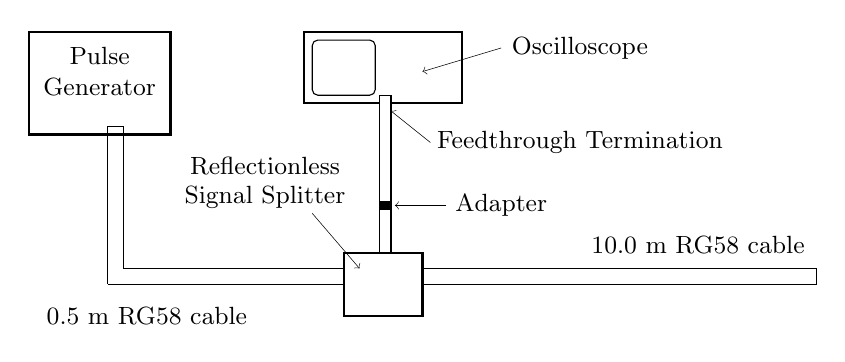
\begin{tikzpicture}
\draw[thin](1,0)--(10,0)--(10,.2)--(1.2,.2)--(1.2,2)--(1,2)--(1,0); %cable
\draw[thick](0,1.9)rectangle(1.8,3.2); %pulse generator
\draw[thick,fill=white](4,-.4)rectangle(5,.4); %signal splitter
\draw[thick,fill=white](3.5,2.3)rectangle(5.5,3.2); %oscilloscope
\draw[rounded corners=2pt](3.6,2.4)rectangle(4.4,3.1); %oscilloscope screen
\draw[fill=white](4.45,.4)rectangle(4.6,2.4); %feedthrough and adapter
\draw[line width=3pt](4.45,1)--(4.6,1);
%labels
\node[font=\small]at(7,3){Oscilloscope};
\draw[very thin,->](6,3)--(5,2.7);
\node[font=\small]at(7,1.8){Feedthrough Termination};
\draw[very thin,->](5.1,1.8)--(4.6,2.2);
\node[font=\small]at(6,1){Adapter};
\draw[very thin,->](5.3,1)--(4.65,1);
\node[font=\small]at(8.5,.5){10.0 m RG58 cable};
\node[font=\small]at(3,1.5){Reflectionless};
\node[font=\small]at(3,1.1){Signal Splitter};
\draw[very thin,->](3.6,.9)--(4.2,.2);
\node[font=\small]at(1.5,-.4){0.5 m RG58 cable};
\node[font=\small]at(.9,2.9){Pulse};
\node[font=\small]at(.9,2.5){Generator};
\end{tikzpicture}
\caption{A diagram of the experimental set up.}
\label{fig:tw1}
\end{figure}

\item Remove the short circuit termination and connect the variable resistor termination. Adjust the resistor until there is no reflection. Remove the variable termination from the circuit and use the Fluke meter to measure its resistance. This is the value for the characteristic impedance of RG58 cable. Now vary the resistance over its entire range. At each point measure the resistance of the termination and the corresponding amplitude of the initial and reflected waves. Take enough data so that you will be able to verify or refute Equation \ref{equ:tw11}.

\item Remove the variable resistance and leave the cable end open. Increase the pulse width until the outgoing pulse overlaps the reflected pulse. Draw a diagram and take amplitude measurements that will allow you to verify or refute the principle of superposition. Decrease the pulse width back to minimum.

\item Connect the 7.0 m RG59 cable to the end of the RG58 cable. Terminate the open end with a short. Sketch what you observe. Describe what each reflected wave represents. Apply the variable resistive termination to the end of the RG59 cable to measure its characteristic impedance. Repeat with the 7.0 m twinaxial cable. %Measure the velocity of propagation. Repeat with the 7.0 m twinaxial cable. Take enough amplitude data so that you can determine which cable type is lossier, RG59 or twinaxial.

\item Set up the circuit shown in Figure \ref{fig:tw2}. Connect one end of the 10.0 m RG58 cable to the t-splitter (connected to channel 1) and the other end to channel 2 of the oscilloscope via the feedthrough termination. Set the oscilloscope display to show both channels 1 and 2 and record the voltage differences between the direct output of the pulse generator and the attenuated signal from the cable. Next, measure the time separation between each pulse to determine the phase velocity of the cable. Repeat with the RG59 and twinaxial cables.

\begin{figure}
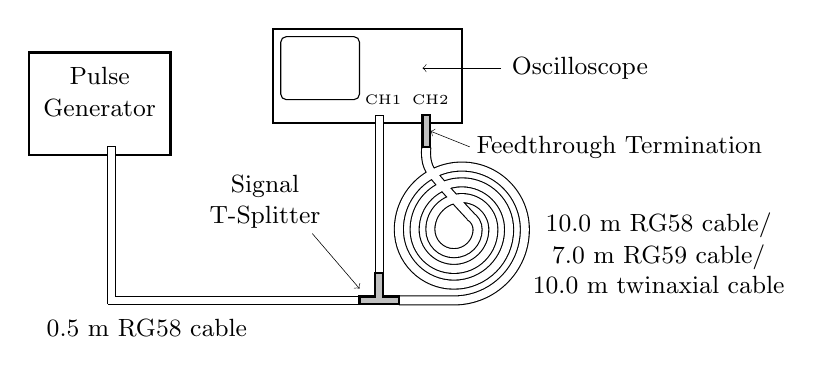
\begin{tikzpicture}
\draw[thick](0,1.9)rectangle(1.8,3.2); %pulse generator
\draw[thin,fill=white](1,0)--(4.2,0)--(4.2,.1)--(1.1,.1)--(1.1,2)--(1,2)--(1,0); %cable
\draw[double distance=.1cm](4.7,.05)--(5.4,.05)arc(270:360:.9)arc(0:180:.8)arc(180:360:.7)
arc(0:180:.6)arc(180:360:.5)arc(0:180:.4)arc(180:360:.3)arc(0:60:.2) 
plot [smooth] coordinates {(5.62,1.11) (5.1,1.7) (5.05,2)}; %cable to be tested
\draw[thick,fill=white](3.1,2.3)rectangle(5.5,3.5); %oscilloscope
\draw[rounded corners=2pt](3.2,2.6)rectangle(4.2,3.4); %oscilloscope screen
\draw[fill=lightgray,thick](5,2)rectangle(5.1,2.4); %feedthrough to CH2
\draw[fill=white](4.4,.2)rectangle(4.5,2.4); %to CH1
\draw[thick,fill=lightgray](4.2,.1)--(4.4,.1)--(4.4,.4)--(4.5,.4)--(4.5,.1)--(4.7,.1)--(4.7,0)
--(4.2,0)--cycle; %splitter
%labels
\node[font=\small]at(7,3){Oscilloscope};
\draw[very thin,->](6,3)--(5,3);
\node[font=\small]at(7.5,2){Feedthrough Termination};
\draw[very thin,->](5.6,2)--(5.1,2.2);
\node[font=\tiny]at(5.1,2.6){CH2};
\node[font=\tiny]at(4.5,2.6){CH1};
\node[font=\small]at(8,1){10.0 m RG58 cable/};
\node[font=\small]at(8,.6){7.0 m RG59 cable/};
\node[font=\small]at(8.,.25){10.0 m twinaxial cable};
\node[font=\small]at(3,1.5){Signal};
\node[font=\small]at(3,1.1){T-Splitter};
\draw[very thin,->](3.6,.9)--(4.2,.2);
\node[font=\small]at(1.5,-.3){0.5 m RG58 cable};
\node[font=\small]at(.9,2.9){Pulse};
\node[font=\small]at(.9,2.5){Generator};
\end{tikzpicture}
\caption{A diagram of the experimental set up for the determination of signal attenuation in RG58, RG59, and twinaxial cables.}
\label{fig:tw2}
\end{figure}

\end{enumerate}
\section{Error Analysis}

The uncertainty in measuring the voltage and the time of the wave is the instrument error of the oscilloscope. Assume that the scale on the oscilloscope screen is a ruler. Then the error is one half of the smallest division. Each division in the horizontal direction will have a size determined by the horizontal oscilloscope setting. Similarly, a vertical division is determined by the vertical oscilloscope setting. Take the length of each cable to be exact. For the multimeter, the error is the instrument error as written on the underside of the meter. 

\section{To be handed in to your laboratory instructor}

%%% begin prelab %%%
\section{Prelab}
\begin{enumerate}

\item Look up values for the characteristic impedance, $Z_0$, and propagation velocity, $V_p$, of RG58 and RG59 cable.

\end{enumerate}
%%% end prelab %%%

\section{{\bf Data Requirements}}
\begin{enumerate}[resume]

\item Two diagrams with measurements and errors that show a single pulse at high time resolution and multiple pulses at lower time resolution for the case of a  direct connection between the pulse generator and the oscilloscope. The y axis is voltage and the horizontal axis is time. 

{\it Note: When producing diagrams from the output of the oscilloscope be sure to record the time and voltage scale settings from the oscilloscope so that fiducial markers may be interpreted correctly for reporting of time and voltage differences.}

\item Two diagrams with measurements and errors that illustrate reflections from an open end and a shorted end in the RG58 cable. Explain whether or not  your measurements agree with the predictions of the theory.

\item A value with error for $Z_0$ and $V_p$ for the RG58, RG59, and twinaxial cables as well as a value for attenuation for the RG58 cable. The units of characteristic impedance are Ohms. Express the velocity of propagation as a percentage of the speed of light. Express the attenuation in percentage loss per meter of cable.

\item Knowing $V_p$, add a horizontal position axis to the figures in part 2 so the waves are known in time and space. How wide is the pulse generator pulse in nanoseconds and in meters?

\item A table of values for the variable resistive termination. Include, termination resistance, forward voltage, reflected voltage, measured reflection coefficient, and expected reflection coefficient. To get a more realistic value for the measured reflection coefficient use your data for loss in the RG58 cable to determine better values for the forward and reflected voltage at the terminated cable end.

\item A diagram along with measurements and errors for the case where the outgoing pulse is superimposed on the reflected pulse.

\item Two diagrams for the observed pulses when the RG59 and twinaxial cables are connected to the end of the RG58. No measurements are needed but you need to explain the source for each of the reflections that you observe. 

\section{Discussion}

\item A comparison between the measured and expected values for the characteristic impedance and velocity of propagation of RG58 and RG59 cables.

\item Using the results of procedure step 4, discuss whether your results support or refute Equation \ref{equ:tw11}. 

\item Using the results of procedure step 5, discuss whether your results support the principle of superposition for signals in the cable.

\item Discuss in a paragraph one of the following.

\begin{enumerate}[label=\Alph*)]

\item Technicians who must repair undersea or buried cables use an instrument called a {\bf time-domain reflectometer} (TDR) to find where the cable is cut. TDR uses traveling waves to find cable breaks. Using traveling wave ideas describe how you would find a cable break. Include a hypothetical example together with some numeric calculations.

\item Traveling wave ideas also apply to the flow of automobile traffic. What would a change in the characteristic impedance be caused by? On the highway you encounter a sudden slowdown and shortly thereafter traffic resumes normal speed. No accident or obstruction is anywhere in sight. What has just happened?

\item To characterize large explosions, including nuclear ones, the position and time of the blast front needs to be measured. One way to do this is to have a collapsible cable that crushes flat as the blast moves along. The collapsing end represents a shorted termination that moves along with the explosion. How would you measure the advancing shock front using traveling waves in such a cable?

\end{enumerate}
\end{enumerate}




\AtEndDocument{\clearpage\ifodd\value{page}\else\null\clearpage\fi} % forces even page count, for double siding

%%%%%%%%%%%%%%%%%%%%%%%%%%%%%%%%%%%%%%%%%%%%%
%
% 0062 PHYS397FA2017 - Companion Guide
%
%%%%%%%%%%%%%%%%%%%%%%%%%%%%%%%%%%%%%%%%%%%%%


\chapter{Travelling Waves - Companion Guide}

\section{Equipment}

% first column
\begin{minipage}[t]{0.5\textwidth}
\begin{itemize}[noitemsep]
\item Tek 2225 oscilloscope with BNC feedthrough termination
\item HP 8011A pulse generator
\item Fluke multimeter
\item 10 meter RG58 coaxial cable
\item 7 meter RG59 coaxial cable
\item 7 meter twinaxial cable
\item reflectionless signal splitter
\end{itemize}
\end{minipage}
%second column
\begin{minipage}[t]{0.5\textwidth}
\begin{itemize}[noitemsep]
\item 0.5 meter RG58 coaxial cable
\item BNC male-male adapter (2)
\item BNC female-female adapter
\item male BNC to female banana adapter
\item banana connecting cables (2)
\item variable resistive termination
\item short circuit termination
\end{itemize}
\end{minipage}

\section{Setup}
\begin{figure}
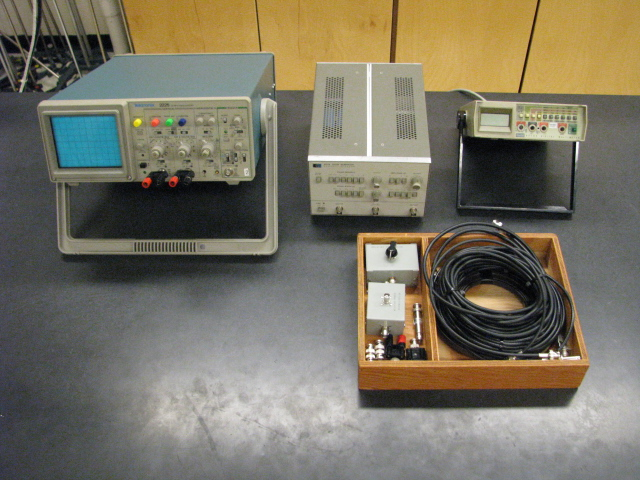
\includegraphics{/usr/local/master/labs/physics397-FA2017/0062-PHYS397FA2017/Travelling-Waves-Setup.jpg}
\caption{Equipment Setup}
\label{pic:TWsetup}
\end{figure}

Set up bench as shown in Figure \ref{pic:TWsetup}.

\section{Maintenance}

\begin{enumerate}
\item 
\item 
\end{enumerate}

\section{Critical Points of Failure}

There are currently no known critical points of failure.

\begin{marginfigure}
\begin{tikzpicture}
%\draw[very thin](0,0)rectangle(11,8);
\node[scale=1.23,opacity=.6]at(5.4,4){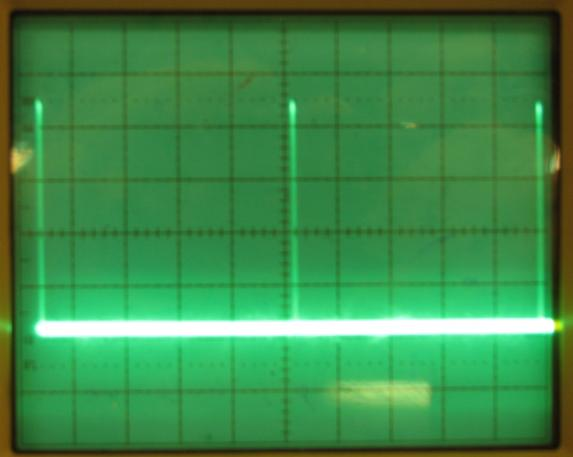
\includegraphics{/usr/local/master/labs/physics397-FA2017/0062-PHYS397FA2017/pulse-low-res.jpg}};
\draw[domain=2.4:8.4,very thin]plot[samples=600](\x,{(2.5*exp(-(\x-5.5)^2/.005))+
(2.5*exp(-(\x-2.7)^2/.005))+(2.5*exp(-(\x-8.2)^2/.005))+2.9});
\draw[thick](2.7,5.6)--(5.5,5.6);
\draw[thick](2.7,5.5)--(2.7,5.7);
\draw[thick](5.5,5.5)--(5.5,5.7);
\draw[thick](5.8,5.4)--(5.8,3);
\draw[thick](5.7,3)--(5.9,3);
\draw[thick](5.7,5.4)--(5.9,5.4);
%math
\node[]at(4.1,5.8){$8.4\pm1.0\mu s$};
\node[]at(4.1,5.3){$1680\pm200.0m$};
\node[right]at(5.8,4.4){$8.4\pm1.0 $ V};
\end{tikzpicture}
\caption{Sketch of pulse train with measurements and uncertainties taken from oscilloscope trace (shown as transparency).}
\label{fig:twcg1}
\end{marginfigure}



\begin{marginfigure}
\begin{tikzpicture}
%\draw[very thin](0,0)rectangle(11,8);
\node[scale=1.2,opacity=.6]at(5.6,4){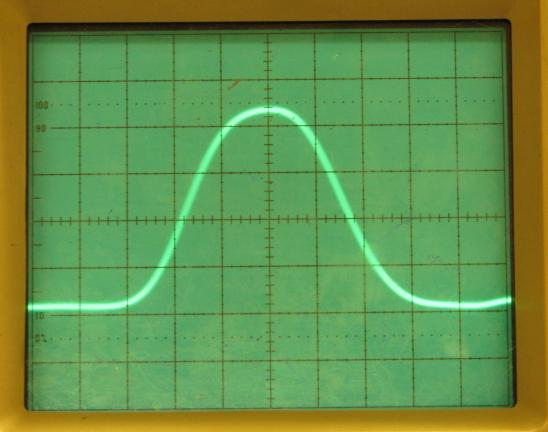
\includegraphics{/usr/local/master/labs/physics397-FA2017/0062-PHYS397FA2017/pulse-high-res.jpg}};

\draw[thick](4,5.6)--(5.6,5.6);
\draw[thick](4,5.5)--(4,5.7);
\draw[thick](5.6,5.5)--(5.6,5.7);
\draw[thick](5.6,2.8)--(7.4,2.8);
\draw[thick](5.6,2.7)--(5.6,2.9);
\draw[thick](7.4,2.7)--(7.4,2.9);

\draw[thick](7,5.2)--(7,3);
\draw[thick](6.9,3)--(7.1,3);
\draw[thick](6.9,5.2)--(7.1,5.2);

\draw[thick](4.8,4.2)--(6.4,4.2);
\draw[thick](4.8,4.1)--(4.8,4.3);
\draw[thick](6.4,4.1)--(6.4,4.3);
%math
\node[]at(4.8,5.3){$0.017\pm0.0025\mu s$};
\node[]at(6.5,2.4){$0.019\pm0.0025\mu s$};
\node[]at(5.6,3.8){$0.0175\pm0.0025\mu s$};
\node[right]at(7,4.4){$8.4\pm1.0 $ V};
\node[]at(4.8,5){$3.40\pm0.5m$};
\node[]at(6.5,2.1){$3.50\pm0.5m$};
\node[]at(5.6,3.5){$3.80\pm0.5m$};
\end{tikzpicture}
\caption{Sketch of single pulse with measurements and uncertainties taken from oscilloscope trace (shown as transparency).}
\label{fig:twcg2}
\end{marginfigure}

\section{Notes to the Instructor}
\begin{enumerate}
\item While making observations and measurements, students should be reminded to keep their body parts away from the cables, splitters, oscilloscope, function generator, and multimeter as proximity can cause large fluctuations in readings on the oscilloscope.
\item Students should remember that when utilizing the 10x magnification feature on the oscilloscope they must divide the horizontal scale value on the {\it sec/div} selector by 10 to obtain time measurements. 
\end{enumerate}

\section{Prelab Questions}
\begin{enumerate}
\item The characteristic impedance for RG58 and RG 59 coaxial cable is Z$_0$=50 $\Omega$ and Z$_0$=75 $\Omega$, respectively. They each have a phase velocity, V$_p$=0.66c, where c is the speed of light in a vacuum.

See http://www.belden.com/resourcecenter/tools/cablefinder.
\end{enumerate}



\section{Data Requirements}
\begin{enumerate}
\item {\bf Two diagrams with measurements and errors that show a single pulse at high time resolution and multiple pulses at lower time resolution for the case of a  direct connection between the pulse generator and the oscilloscope. The y axis is voltage and the horizontal axis is time.}\newline

Figures \ref{fig:twcg1} and \ref{fig:twcg2} show the oscilloscope traces for a pulse train and single pulse, respectively. Measurements are read off the oscilloscope screen and have been included in the figures.


\item {\bf Two diagrams with measurements and errors that illustrate reflections from an open end and a shorted end in the RG58 cable. Explain whether or not  your measurements agree with the predictions of the theory.}\newline

Figures \ref{fig:twcg3} and \ref{fig:twcg4} show the oscilloscope traces for a wave reflected at an open termination and a shorted termination, respectively. Measurements of peak voltage for both cases show that they differ by sign only. This agrees with the theory of reflections at these types of boundaries.

\begin{marginfigure}
\begin{tikzpicture}
%\draw[very thin](0,0)rectangle(11,8);
\node[scale=1.2,opacity=.8]at(5.5,4){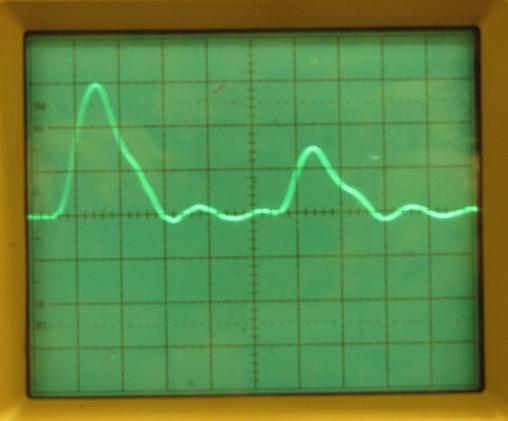
\includegraphics{/usr/local/master/labs/physics397-FA2017/0062-PHYS397FA2017/open-end-reflection.jpg}};

\draw[thick](3.7,3.7)--(6.2,3.7);
\draw[thick](3.7,3.6)--(3.7,3.8);
\draw[thick](6.2,3.6)--(6.2,3.8);

\draw[thick](3.9,3.9)--(3.9,5.5);
\draw[thick](3.8,3.9)--(4,3.9);
\draw[thick](3.8,5.5)--(4,5.5);

\draw[thick](6.5,3.95)--(6.5,4.8);
\draw[thick](6.4,3.95)--(6.6,3.95);
\draw[thick](6.4,4.8)--(6.6,4.8);

%math
\node[]at(5,5){$2.5\pm0.25$ V};
\node[]at(5.,3.3){$0.102\pm0.01\mu s$};
\node[]at(7.4,4.4){$1.3\pm.25$ V};
\end{tikzpicture}
\caption{Open end reflection.}
\label{fig:twcg3}
\end{marginfigure}


\begin{marginfigure}
\begin{tikzpicture}
%\draw[very thin](0,0)rectangle(11,8);
\node[scale=1.2,opacity=.9]at(5.5,4){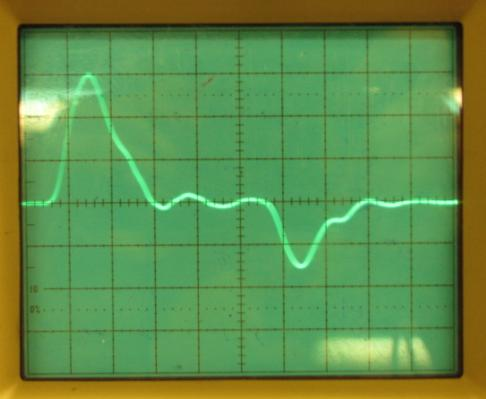
\includegraphics{/usr/local/master/labs/physics397-FA2017/0062-PHYS397FA2017/shorted-reflection.jpg}};

\draw[thick](3.7,2.9)--(6.2,2.9);
\draw[thick](3.7,2.8)--(3.7,3);
\draw[thick](6.2,2.8)--(6.2,3);

\draw[thick](3.9,3.9)--(3.9,5.5);
\draw[thick](3.8,3.9)--(4,3.9);
\draw[thick](3.8,5.5)--(4,5.5);

\draw[thick](6.5,4)--(6.5,3.15);
\draw[thick](6.4,4)--(6.6,4);
\draw[thick](6.4,3.15)--(6.6,3.15);

%math
\node[]at(5,5){$2.5\pm0.25$ V};
\node[]at(5.,2.4){$0.102\pm0.01\mu s$};
\node[]at(7.4,3.4){$1.3\pm.25$ V};
\end{tikzpicture}
\caption{Shorted end reflection.}
\label{fig:twcg4}
\end{marginfigure}


\item {\bf A value with error for $Z_0$ and $V_p$ for the RG58, RG59, and twinaxial cables as well as a value for attenuation for the RG58 cable. The units of characteristic impedance are Ohms. Express the velocity of propagation as a percentage of the speed of light. Express the attenuation in percentage loss per meter of cable.}\newline

The phase velocity is found (for the RG58 cable) as follows

\begin{equation}
V_p=\dfrac{2\ell}{t}=\dfrac{20m}{0.102\mu s}=0.654c
\label{}
\end{equation}

\noindent Where $\ell$ is the length of the cable and $t$ is the time between the forward and reflected pulses. The uncertainty is then,

\begin{equation}
u(V_p)=\dfrac{2\ell}{t^2}\cdot u(t)=\dfrac{20m}{(0.102\mu s)^2}\cdot 0.01\mu s=0.064c
\label{}
\end{equation}

\noindent The RG59's phase velocity is found likewise to be the same value.

The characteristic impedance of each cable is determined from the variable resistor and multimeter. Given that there is uncertainty in the oscilloscope reading of the zero-reflection impedance in addition to the uncertainty in the multimeter we take the uncertainty in the measurement to be $\pm$2 $\Omega$. The characteristic impedances of the RG58 and RG59 cables are then 49.7$\pm$2 $\Omega$ and 76.4$\pm$2 $\Omega$, respectively.

The attenuation of a signal in the wire is like compounding interest. Through every meter of cable, a percentage of the initial signal is dissipated so that, at the start of the next meter, the initial voltage is less than at the beginning and a percentage of {\it that} voltage is dissipated. The formula for this type of compounding loss is

\begin{equation}
V_f=V_0(1-p)^n
\label{}
\end{equation}

\noindent where $n$ is the length in meters, $p$ is the fraction of signal lost after each meter, $V_0$ is the initial voltage, and $V_f$ is the voltage of the signal at the end of the $n$-meter cable. We can then find an expression for $p$.

\begin{equation}
p=1-\left(\dfrac{V_f}{V_0}\right)^{\frac{1}{n}}
\label{}
\end{equation}

The uncertainty in this attenuation value is found with the following partial derivative


\begin{equation}
u(p)=\sqrt{\left(-\dfrac{u(V_f)}{nV_0} \left(\dfrac{V_f}{V_0}\right)^{\frac{1}{n}-1}\right)^2+\left(-\dfrac{V_fu(V_0)}{nV_0^2} \left(\dfrac{V_f}{V_0}\right)^{\frac{1}{n}-1}\right)^2}
\label{}
\end{equation}



Using these expressions we find that the attenuation in the RG58 and RG59, expressed as percent loss per meter, is 1.11\%/m and 3.55\%/m, respectively.

\item {\bf Knowing $V_p$, add a horizontal position axis to the figures in part 2 so the waves are known in time and space. How wide is the pulse generator pulse in nanoseconds and in meters?}\newline

We can find spacial width using the relationship $\Delta x=V_p\Delta t$, where V$_p$=0.66c. The uncertainty is then $u(x)=V_p\cdot u(t)$. These computed values have been included in Figures \ref{fig:twcg1} and \ref{fig:twcg2}. The pulse is 17.5 ns and 3.80 m in width.

\item {\bf A table of values for the variable resistive termination. Include, termination resistance, forward voltage, reflected voltage, measured reflection coefficient, and expected reflection coefficient. To get a more realistic value for the measured reflection coefficient use your data for loss in the RG58 cable to determine better values for the forward and reflected voltage at the terminated cable end.}\newline

Table \ref{tab:twcg1} includes values for termination resistance, R$_T$, forward voltage, v$_+$, reflected voltage, v$_-$, measured reflection coefficient, $\Gamma_m$, attenuation-corrected reflection coefficient, $\Gamma_{corr}$, and the expected reflection coefficient, $\Gamma_{theory}$.

Because the voltage measurements were made with the oscilloscope, their associated uncertainties are half the larger divisions which, in this case, are $\pm$0.1 V.

The uncertainty in resistance measurements obtained through the use of the Fluke multimeter is $\pm0.2\%+ 1$ digit.

The attentuation-corrected reflection coefficient is simply the measured value divided by the percent voltage loss in 20 m of cable. Note that the pulse travels the length of the 10 m cable twice for a return trip to the oscilloscope. The uncertainty in the reflection coefficient must be found by the partial derivative method (shown below) or by an acceptable approximation to it.

Figure \ref{fig:twcg5} plots the calculated reflection coefficient from Table \ref{tab:twcg1} vs. impedance. It can easily be seen that when impedance is zero, the reflection coefficient is -1 and when it tends towards infinity the coefficient is 1. The reflection coefficient is also zero when the variable resistor is set to be identical to the characteristic impedance of the cable, i.e., 50 $\Omega$.

\begin{figure}
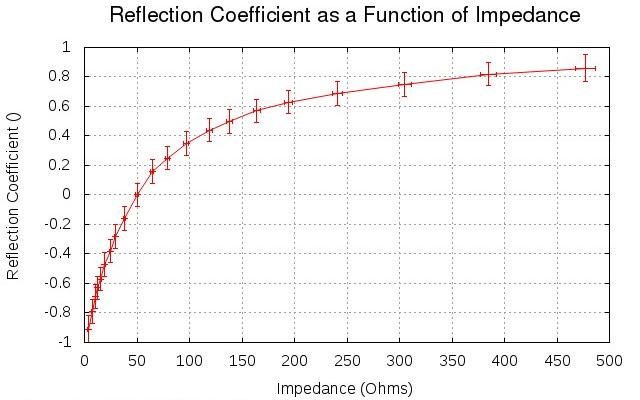
\includegraphics{/usr/local/master/labs/physics397-FA2017/0062-PHYS397FA2017/VarResistor.jpg}
\caption{A plot of reflection coefficient vs. impedance.}
\label{fig:twcg5}
\end{figure}

\begin{equation}
\Gamma_m=\dfrac{v_-}{v_+}
\label{equ:twcg1}
\end{equation}

\begin{align}
u(\Gamma_m)&=\sqrt{(\dfrac{\partial \Gamma_m}{\partial v_-}\cdot u(v_-))^2+(\dfrac{\partial \Gamma_m}{\partial v_+}\cdot u(v_+))^2}\\
&=\sqrt{(\dfrac{u(v_-)}{v_+})^2+(\dfrac{v_-}{v_+^2}\cdot u(v_+))^2}
\label{equ:twcg2}
\end{align}

\begin{equation}
\Gamma_{corr}=\dfrac{\Gamma_m}{0.48}
\label{equ:twcg3}
\end{equation}

\begin{equation}
u(\Gamma_{corr})=\dfrac{1}{0.48}\cdot u(\Gamma_m)
\label{equ:twcg4}
\end{equation}


\begin{maintable}[ht]
\begin{tabular}{|l|l|l|l|l|l|}
\hline
\multicolumn{1}{|c|}{$R_T$ ($\Omega$)} & \multicolumn{1}{c|}{v$_+$ (V)} & \multicolumn{1}{c|}{v$_-$ (V)} & \multicolumn{1}{c|}{$\Gamma_m$} & \multicolumn{1}{c|}{$\Gamma_{corr}$} & \multicolumn{1}{c|}{$\Gamma_{theory}$} \\ \hline
$477\pm9.64$                           & $2.65\pm0.1$                   & $1.10\pm0.1$                   & $0.42\pm0.04$                   & $0.86\pm0.09$                        & 0.81                                   \\ \hline
$385\pm7.80$                           & $2.65\pm0.1$                   & $1.04\pm0.1$                   & $0.39\pm0.04$                   & $0.82\pm0.08$                        & 0.77                                   \\ \hline
$305\pm6.20$                           & $2.65\pm0.1$                   & $0.96\pm0.1$                   & $0.36\pm0.04$                   & $0.75\pm0.08$                        & 0.72                                   \\ \hline
$241\pm4.92$                           & $2.65\pm0.1$                   & $0.88\pm0.1$                   & $0.33\pm0.04$                   & $0.69\pm0.08$                        & 0.66                                   \\ \hline
$194\pm3.98$                           & $2.65\pm0.1$                   & $0.80\pm0.1$                   & $0.30\pm0.04$                   & $0.63\pm0.08$                        & 0.59                                   \\ \hline
$164\pm3.38$                           & $2.65\pm0.1$                   & $0.72\pm0.1$                   & $0.27\pm0.04$                   & $0.57\pm0.08$                        & 0.53                                   \\ \hline
$138\pm2.86$                           & $2.65\pm0.1$                   & $0.64\pm0.1$                   & $0.24\pm0.04$                   & $0.50\pm0.08$                        & 0.47                                   \\ \hline
$119\pm2.48$                           & $2.65\pm0.1$                   & $0.56\pm0.1$                   & $0.21\pm0.04$                   & $0.44\pm0.08$                        & 0.41                                   \\ \hline
$96.7\pm2.03$                          & $2.65\pm0.1$                   & $0.44\pm0.1$                   & $0.17\pm0.04$                   & $0.35\pm0.08$                        & 0.32                                   \\ \hline
$79.0\pm1.68$                          & $2.65\pm0.1$                   & $0.32\pm0.1$                   & $0.12\pm0.04$                   & $0.25\pm0.08$                        & 0.22                                   \\ \hline
$64.6\pm1.39$                          & $2.65\pm0.1$                   & $0.20\pm0.1$                   & $0.08\pm0.04$                   & $0.16\pm0.08$                        & 0.13                                   \\ \hline
$50.1\pm1.10$                          & $2.65\pm0.1$                   & $0.00\pm0.1$                   & $0.00\pm0.04$                   & $0.00\pm0.08$                        & 0.00                                   \\ \hline
$38.3\pm0.87$                          & $2.65\pm0.1$                   & $-0.20\pm0.1$                  & $-0.08\pm0.04$                  & $-0.16\pm0.08$                       & -0.13                                  \\ \hline
$29.3\pm0.69$                          & $2.65\pm0.1$                   & $-0.32\pm0.1$                  & $-0.14\pm0.04$                  & $-0.28\pm0.08$                       & -0.26                                  \\ \hline
$24.5\pm0.59$                          & $2.65\pm0.1$                   & $-0.48\pm0.1$                  & $-0.18\pm0.04$                  & $-0.38\pm0.08$                       & -0.34                                  \\ \hline
$19.4\pm0.49$                          & $2.65\pm0.1$                   & $-0.60\pm0.1$                   & $-0.23\pm0.04$                  & $-0.47\pm0.08$                       & -0.44                                  \\ \hline
$15.4\pm0.41$                          & $2.65\pm0.1$                   & $-0.72\pm0.1$                  & $-0.27\pm0.04$                  & $-0.57\pm0.08$                       & -0.53                                  \\ \hline
$12.7\pm0.35$                          & $2.65\pm0.1$                   & $-0.80\pm0.1$                  & $-0.30\pm0.04$                  & $-0.63\pm0.08$                       & -0.60                                  \\ \hline
$10.4\pm0.31$                          & $2.65\pm0.1$                   & $-0.88\pm0.1$                  & $-0.33\pm0.04$                  & $-0.69\pm0.08$                       & -0.66                                  \\ \hline
$7.20\pm0.24$                          & $2.65\pm0.1$                   & $-1.00\pm0.1$                  & $-0.38\pm0.04$                  & $-0.79\pm0.08$                       & -0.75                                  \\ \hline
$3.40\pm0.17$                          & $2.65\pm0.1$                   & $-1.16\pm0.1$                  & $-0.44\pm0.04$                  & $-0.91\pm0.09$                       & -0.87                                  \\ \hline
\end{tabular}
\caption{A table of values for the investigation of variable termination resistance and the behaviour of reflected waves.}
\label{tab:twcg1}
\end{maintable}



\item {\bf A diagram along with measurements and errors for the case where the outgoing pulse is superimposed on the reflected pulse.}\newline

See Figure \ref{fig:twcg6}.

\begin{marginfigure}
\begin{tikzpicture}
\node[above right,scale=1.15]at(0,0){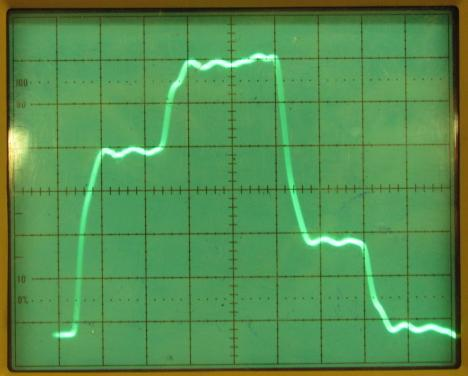
\includegraphics{/usr/local/master/labs/physics397-FA2017/0062-PHYS397FA2017/superimposed-reflection.jpg}};
%1st plateau
\draw[thick](1.4,.6)--(1.4,2.9);
\draw[thick](1.3,.6)--(1.5,.6);
\draw[thick](1.3,2.9)--(1.5,2.9);
\node[right,font=\footnotesize]at(1.4,1.8){4.0$\pm$0.5 V};
%2nd plateau
\draw[thick](3,.6)--(3,4.1);
\draw[thick](2.9,4.1)--(3.1,4.1);
\draw[thick](2.9,.6)--(3.1,.6);
\node[right,font=\footnotesize]at(3,2.6){5.9$\pm$1.0 V};
%3rd plateau
\draw[thick](4.5,.6)--(4.5,1.8);
\draw[thick](4.4,.6)--(4.6,.6);
\draw[thick](4.4,1.8)--(4.6,1.8);
\node[right,font=\footnotesize]at(4.4,1.1){1.9$\pm$0.5 V};
\end{tikzpicture}
\caption{An outgoing pulse superimposed upon its reflected pulse.}
\label{fig:twcg6}
\end{marginfigure}

\item {\bf Two diagrams for the observed pulses when the RG59 and twinaxial cables are connected to the end of the RG58. No measurements are needed but you need to explain the source for each of the reflections that you observe.}\newline

Figures \ref{fig:twcg7} and \ref{fig:twcg8} show the oscilloscope trace of the RG59 and twinaxial cables. 

In Figure \ref{fig:twcg7}, point A represents the initial pulse from the generator, B represents the reflection of the signal as it crosses the interface between the 50 $\Omega$ RG58 and the 75 $\Omega$ RG59, C represents the reflection from the terminated end of the RG59, and D represents the returning C signal reflecting again at the interface and the end of the RG59 before returning to the oscilloscope.

In Figure \ref{fig:twcg8}, point A represents the initial pulse from the generator, B represents the reflection from the interface of the RG58 and the twinaxial cables, and C through G represent the reflected signals bouncing between the interface and the shorted end of the twinaxial cable.

\end{enumerate}


\begin{marginfigure}
\begin{tikzpicture}
\node[above right,scale=1.1]at(0,0){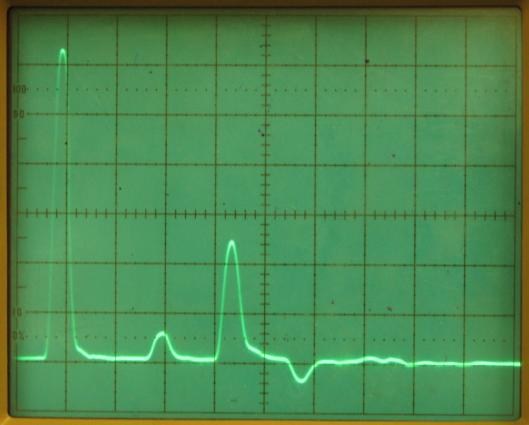
\includegraphics{/usr/local/master/labs/physics397-FA2017/0062-PHYS397FA2017/rg59-open.jpg}};
\node[]at(1,4.3){A};
\node[]at(1.8,1.4){B};
\node[]at(2.6,2.4){C};
\node[]at(3.4,1){D};
\end{tikzpicture}
\caption{10.0 m of RG58 with an additional 7.0 m of RG59, open termination.}
\label{fig:twcg7}
\end{marginfigure}



\begin{marginfigure}
\begin{tikzpicture}
\node[above right,scale=1.1]at(0,0){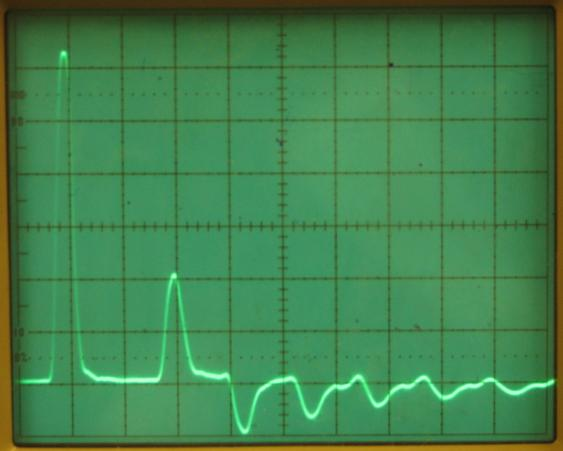
\includegraphics{/usr/local/master/labs/physics397-FA2017/0062-PHYS397FA2017/coax-shorted.jpg}};
\node[]at(1,4.3){A};
\node[]at(1.8,2.2){B};
\node[]at(2.6,1){C};
\node[]at(3.3,1){D};
\node[]at(4,1){E};
\node[]at(4.7,1){F};
\node[]at(5.4,1){G};
\end{tikzpicture}
\caption{10.0 m of RG58 with an additional 7.0 m of twinaxial cable, shorted termination.}
\label{fig:twcg8}
\end{marginfigure}


\section{Discussion}
\begin{enumerate}[resume]

\item {\bf A comparison between the measured and expected values for the characteristic impedance and velocity of propagation of RG58 and RG59 cables.}\newline

Results for the characteristic impedance and phase velocity of RG58 and RG59 coaxial cables can be found in the Data Requirements section. Experimentally determined values match with expected values to within experimental uncertainty. Uncertainty in measurements of the characteristic impedance was taken to be $\pm$2 $\Omega$, much larger than the uncertainties of the oscilloscope reading and multimeter reading combined. This is because of the difficulty in discerning the state of no reflection in the cables. Instead of a straight line at zero Volts one sees an "s-curve" above and below the zero voltage line. Because of this there is a rather large amount of ambiguity in where exactly the variable resistor should be set for the condition of no reflections to be met. Several independent measurements were taken and the resulting variance was taken to be the uncertainty in these measurements.

\item {\bf Using the results of procedure step 4, discuss whether your results support or refute Equation 11. }\newline

We can see from Figure \ref{fig:twcg5} that the reflection coefficient is -1 when the terminating resistance is zero. We then expect to see a reflected pulse of equal-but-negative amplitude and that is indeed what the data indicates. We also see that as the terminating resistance tends toward infinity the reflection coefficient tens toward +1. We then expect to see a reflected pulse of equal-and-positive amplitude and that is, again, what the data indicates. 

These two limiting cases, that of zero and infinite termination resistance, when plugged into Equation 11, give us the expected -1 and +1, respectively.

\item {\bf Using the results of procedure step 5, discuss whether your results support the principle of superposition for signals in the cable.}\newline

From step 5, the two superimposed waves do indeed add up according to the principle of superposition. See Figure \ref{fig:twcg6}.

\item {\bf Discuss in a paragraph one of the following.}

\begin{enumerate}[label=\Alph*)]

\item {\bf Technicians who must repair undersea or buried cables use an instrument called a {\bf time-domain reflectometer} (TDR) to find where the cable is cut. TDR uses traveling waves to find cable breaks. Using traveling wave ideas describe how you would find a cable break. Include a hypothetical example together with some numeric calculations.}\newline

A complete break in an undersea cable would represent a termination in the cable. At this termination, presuming it had an impedance not equal to the characteristic impedance of the cable, one would see a reflection of any signal sent down the line. Knowing the phase velocity of the cable, 0.66c for example, and the time for the reflection to return to a measuring device, let's say 0.1 $\mu$s, one could easily determine the distance along the cable to where the break was by the following computation,

\begin{equation}
d=V_pt=\left(.66\right)\left(3\times10^{8}\right)\left(0.0001\right)=19.8 km
\label{}
\end{equation}

\item {\bf Traveling wave ideas also apply to the flow of automobile traffic. What would a change in the characteristic impedance be caused by? On the highway you encounter a sudden slowdown and shortly thereafter traffic resumes normal speed. No accident or obstruction is anywhere in sight. What has just happened?}\newline

A change in the characteristic impedance of a road could be caused by a narrowing of the road. The sudden slowdown is analagous to a pressure wave, either a reflection or a forward wave, travelling down the line of cars. For instance, a driver up ahead has reactively tapped their brakes causing the person behind them to do the same and so on down the line. The result is a density perturbation travelling down the line to your location.

\item {\bf To characterize large explosions, including nuclear ones, the position and time of the blast front needs to be measured. One way to do this is to have a collapsible cable that crushes flat as the blast moves along. The collapsing end represents a shorted termination that moves along with the explosion. How would you measure the advancing shock front using traveling waves in such a cable?}\newline

The advancing shockwave pins the cable to the ground causing the end of the cable to be terminated with an effectively infinite impedance. If a series of signals are then sent down the line from a safe distance and the time difference of each reflection is recorded, the distance from the origin to the shockwave can be measured as in the undersea cable. If we know the time between each successive signal in the series we can determine a time rate of change for the shockwave.

\end{enumerate}

\end{enumerate}



\AtEndDocument{\clearpage\ifodd\value{page}\else\null\clearpage\fi} % forces even page count, for double siding

\end{document}
